%% Tex spellcheck
% Maybe put this as Chapter 2

% Write in English.
\chapter{Chapter 4 : Testing some coil designs}

We will now test several of the designs discussed in the previous chapter by creating PCBs incorporating these coil designs. Additionally, we will include a driver and control system to regulate the current flowing through the coils.

\section{Existing designs}

To determine the optimal solution for our application, we have tested various existing designs that use PCB coils to move a magnet. For all these tests, we will utilize a driving circuit and a microcontroller mounted on a breadboard.

\subsection{Driver circuit}

In order to control the current in the coils, we will need some driving circuitry. We will use simple NMOS transistors. Leds were added to visually see which coil is activated. The schematics of the driver circuit is shown in figure \ref{fig:breadboard_schematics} and the mounted circuit is shown in figure \ref{fig:breadboard_driver}. Since these coils are inductive, flyback diodes were added to protect the transistors and the power supply.

When setting the GPIOs to a logic high, the transistor will conduct and the current will flow from the power supply to the coil. When setting the GPIOs to a logic low, the transistor will stop conducting.

The same circuit will be used for testing two different existing coil designs.

\begin{figure}[H]
	\centering
	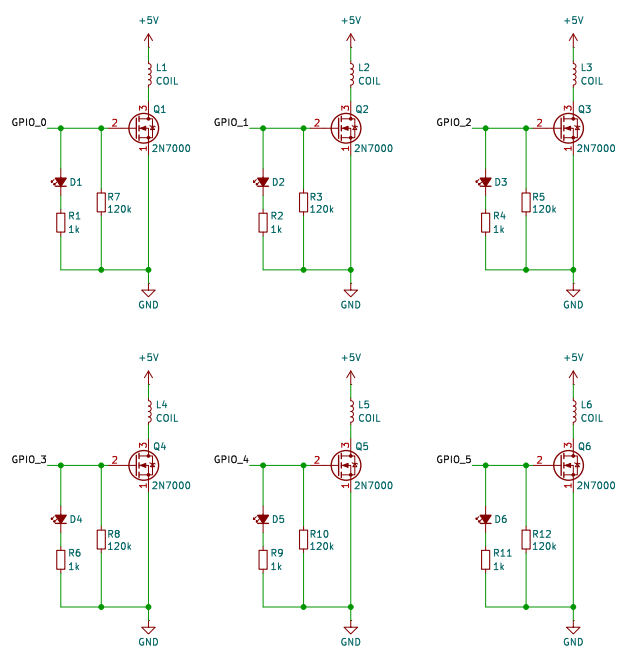
\includegraphics[width=0.7\linewidth]{breadboard_schematics.png}
	\caption[Schematics of the driver breadboard circuit to control the coils]{Schematics of the driver breadboard circuit to control the coils}
	\label{fig:breadboard_schematics}
\end{figure}

\begin{figure}[H]
	\centering
	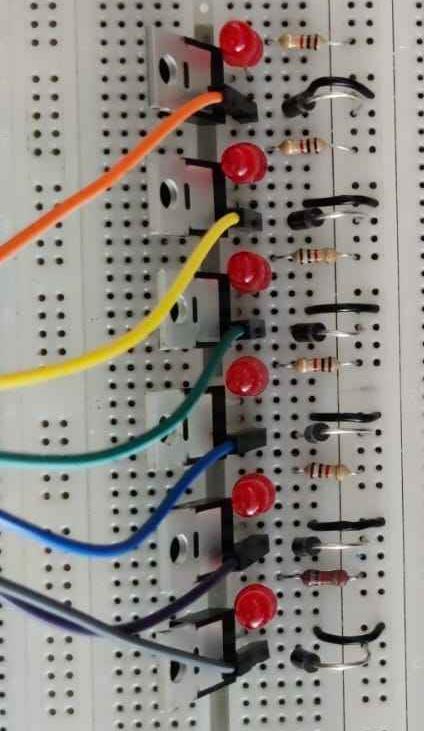
\includegraphics[width=0.6\linewidth, angle=-90]{breadboard_driver.png}
	\caption[Mounted Breadboard circuit]{Mounted Breadboard circuit}
	\label{fig:breadboard_driver}
\end{figure}

\subsection{Control firmware}

For this tests, the coils are controlled via a Raspberry Pi PICO\footcite{ltd_buy_nodate} programmed in MicroPython and six \gls{gpio}s are connected to the transistors and will be used to control the current in the coils. The code is shown in figure \ref{fig:up_code}.

\begin{figure}[H]
	\centering
	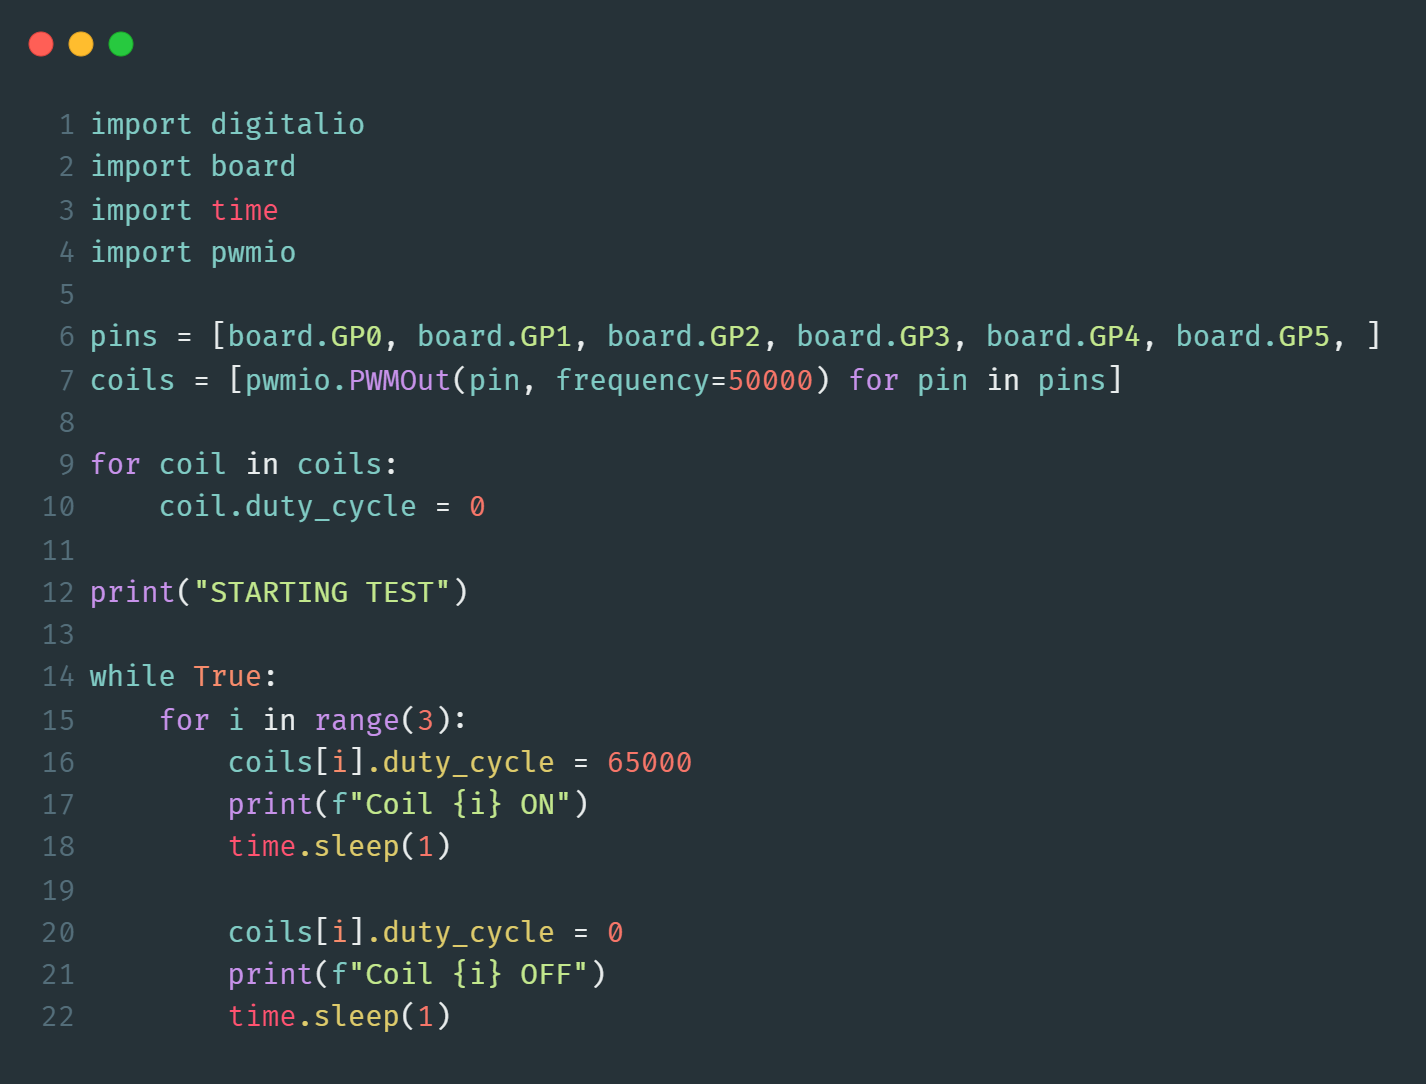
\includegraphics[width=1\linewidth]{code_micropython.png}
	\caption[Micropython code to control the coils with a \gls{pwm}]{Micropython code to control the coils with a \gls{pwm}}
	\label{fig:up_code}
\end{figure}

\subsection{Pemi Technology linear coils}

The first one comes from Pemi Technology\footcite{noauthor_home_nodate} and uses the alternating linear coils. We'll use the driving circuit to control the current in the coils. There is two 4 pin connectors on the \gls{pcb}, one connector for each (X / Y) axis. One of these pins is common to the three coils and will be connected to the power supply, the other three pins are connected to the other side of the coils and will be pulled to ground by transistors to activate the coils.

\begin{figure}[H]
	\centering
	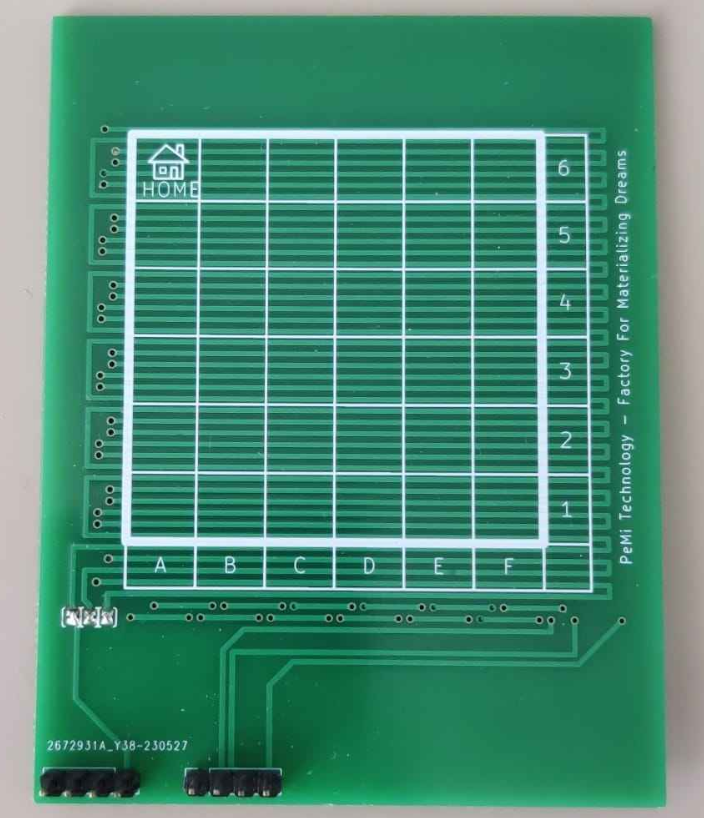
\includegraphics[width=0.5\linewidth]{pemi_linear.png}
	\caption[Pemi Technology linear coils \gls{pcb}]{Pemi Technology linear coils \gls{pcb}}
	\label{fig:pemi_pcb}
\end{figure}

The \gls{pcb} characteristics are:
\begin{itemize}
	\item 3 coils for each axis
	\item 10 mils (0.254mm) spacing between each coil
	\item 20 mils (0.508mm) width for the traces
\end{itemize}

The magnet used for the tests:
\begin{itemize}
	\item 3mmx3mmx3mm cubic magnet
	\item 5mmx5mmx5mm cubic magnet
	\item 2mm diamter round magnet
	\item 2mmx2mmx1mm cubic magnet
\end{itemize}


The tests consist on alternating the activation of the coils and see if we could move a magnets. We used different magnet sizes and shapes to see if we could move them.
\\

We could only move the smallest magnets (2mmx2mm) and only in one axis. The direction was managed by the order of activation of the coils, and changing this order did change the diection. There still was some moments where the magnet would be stuck or moving back and forth on the same three coils.
\\

The axis where the magnet was moving was the one on the top layer of the \gls{pcb}, this means that the coils on the bottom layer were not strong enough to move the magnet bacause they were further to the magnet than the top layer ones.

\subsection{HEPIA linear coils}

In a previous intership\footcite{noauthor_arthurabelkalo_2023}, a \gls{pcb} was designed with the same linear coils concept. It's actually compose of 4 identical board, each with 9x9 cell. These cells should be individually controllable to move a magnet in each sub surface. The \gls{pcb} has some issues, notably all the columns are connected together but should be individually controllable. This renders the final \gls{pcb} unusable for our application.\\

Besides the electrical issues, the \gls{pcb} is made on 6 layers with bind vias, making it very hard to develop, expensive to produce and really hard to debug.

\begin{itemize}
	\item 9x9 cell
	\item 6 layer board
	\item Bind vias
	\item 3 coils for each axis
	\item 0.3mm spacing between each coil
	\item 0.5mm width for the traces
\end{itemize}

\begin{figure}[H]
	\centering
	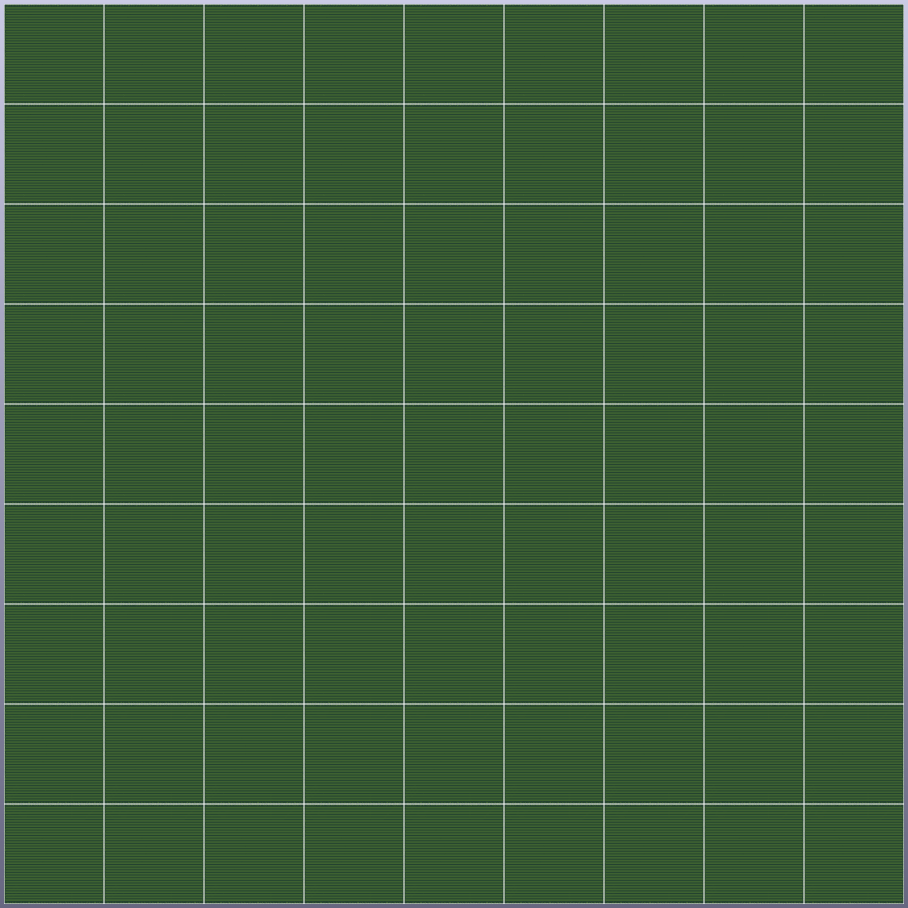
\includegraphics[width=0.6\linewidth]{pcb_stage.png}
	\caption[Intern's \gls{pcb} with linear coils]{\gls{hepia} Intern's \gls{pcb} with linear coils}
	\label{fig:intern_pcb}
\end{figure}

\begin{figure}[H]
	\centering
	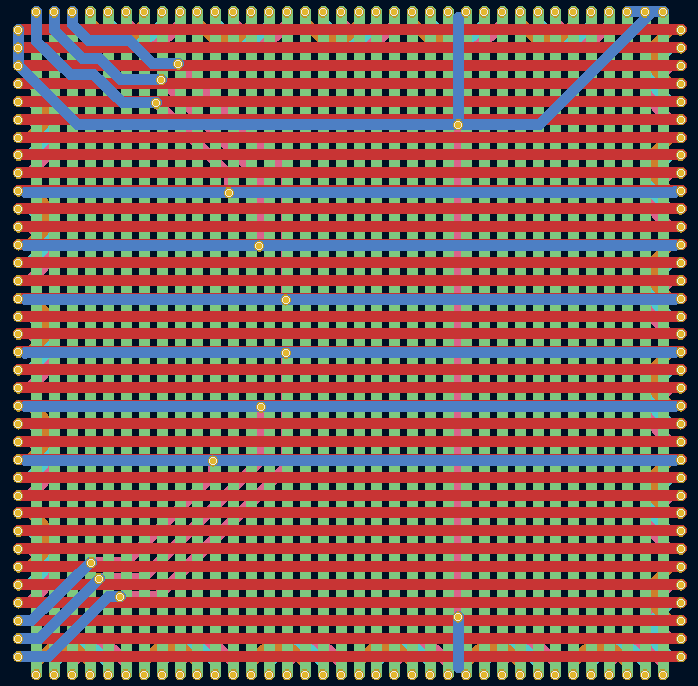
\includegraphics[width=0.6\linewidth]{single_cell_all.png}
	\caption[Single cell intern's \gls{pcb}]{Single cell of the intern's \gls{pcb} with all layers}
	\label{fig:single_cell_all}
\end{figure}


\newpage

\section{Custom PCB to test designs}

In order to test some coil design and to have a better control over the coils while also testing some ways to control the current in the coils, we designed a custom \gls{pcb} with 4 different coil designs. Two of these designs are still linear coils but with different spacing and width. The other two designs are circular coils with different trace width and spacing to see if more turns or more current impacts the magnetic field while keeping the same diameter.

We also wanted to keep the \gls{pcb} as 2 layers to keep the cost down and see if it was enough to move a magnet.

\begin{figure}[H]
	\centering
	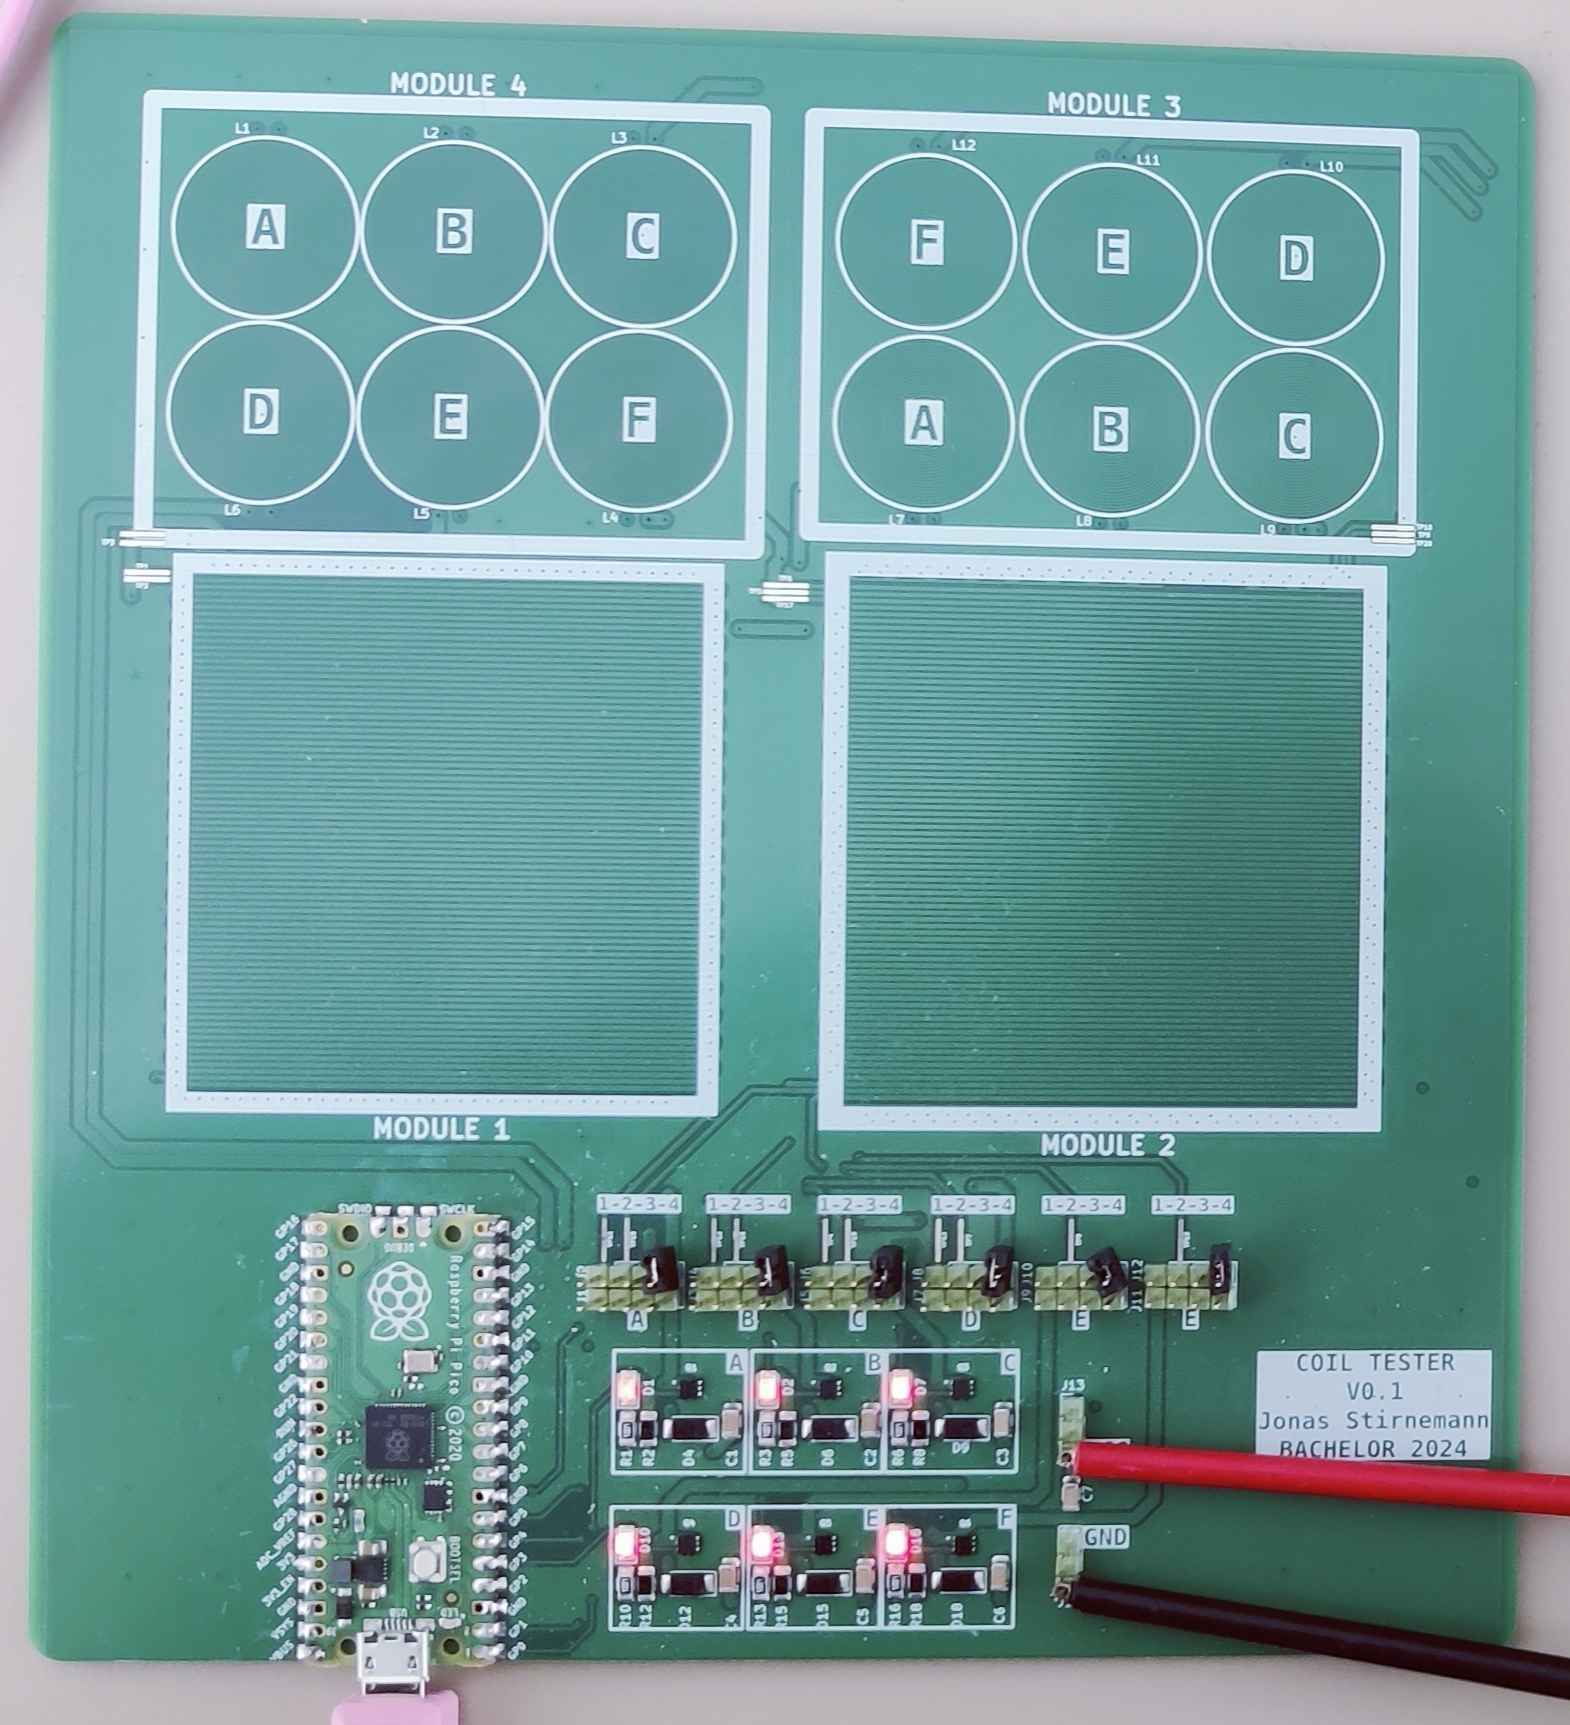
\includegraphics[width=0.8\linewidth]{coil_driver_pcb.jpg}
	\caption[Mounted Custom test \gls{pcb} ]{Mounted custom test \gls{pcb}}
	\label{fig:coil_driver_pcb}
\end{figure}

\begin{figure}[H]
	\centering
	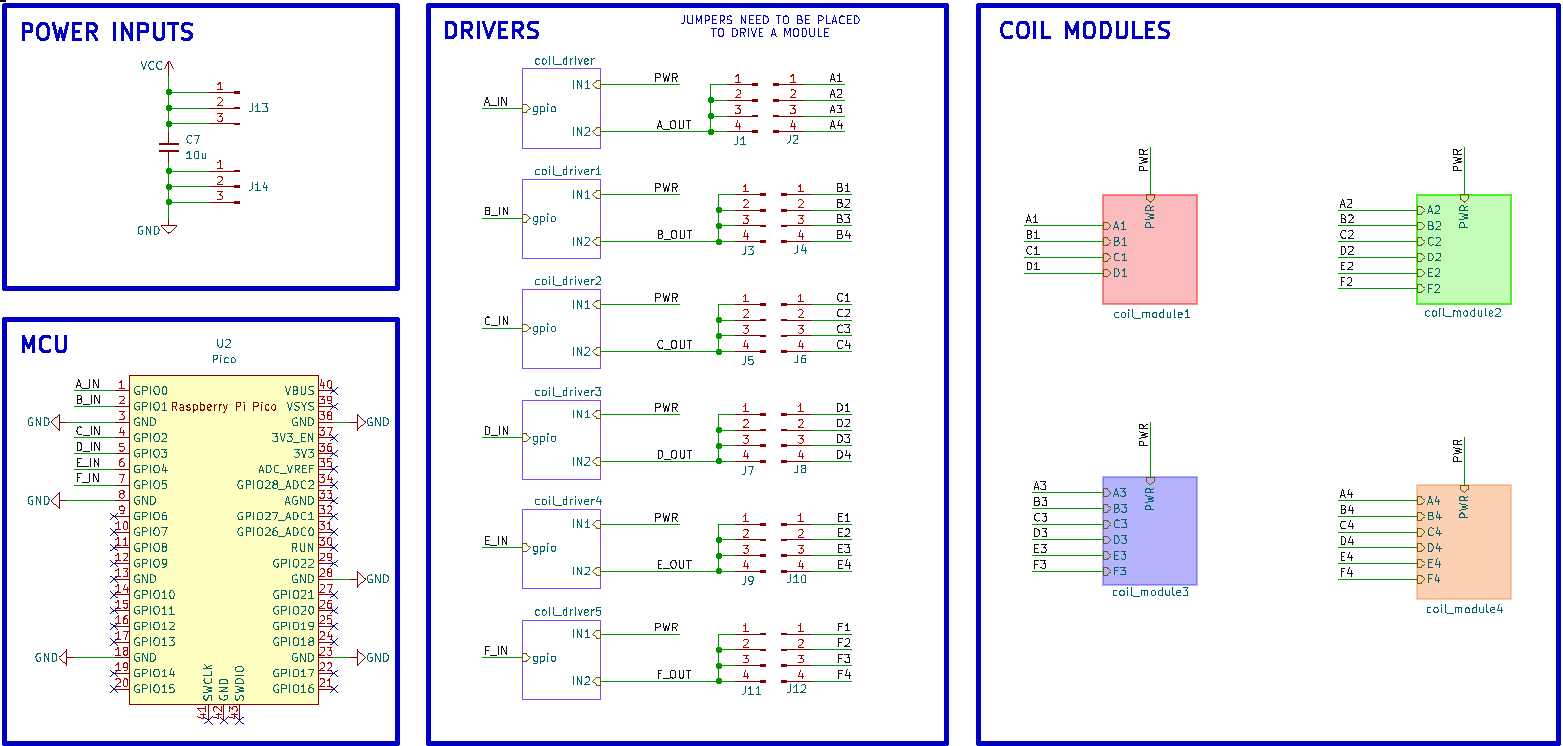
\includegraphics[width=1.4\linewidth, angle=90]{coil_driver_full_schematics.png}
	\caption[Custom test \gls{pcb} general schematics]{Custom test \gls{pcb} general schematics}
	\label{fig:coil_driver_full_schematics}
\end{figure}


\subsection{Driver circuitry}

We would only test one design at the time, so we would only need one driver circuit and we would want to change which coil design is connected to it. For that we simply added pin aligned pin headers so that we can physically connect which design is connected to the driving circuit. One other advantage of this method, is that we can also easily connect any external design on the driving circuit.

\begin{figure}[H]
	\centering
	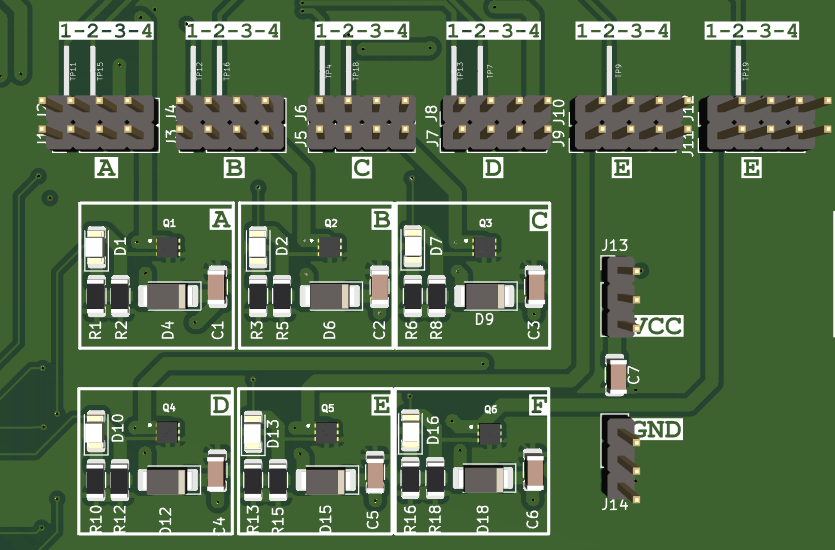
\includegraphics[width=0.5\linewidth]{design_choice.png}
	\caption[Pin header for chosing the driven design]{Pin header for chosing the driven design}
	\label{fig:deisgn_choice}
\end{figure}


The driver part is composed of 6 NMOS transistors and some LEDs to visually see which coil is activated.

\begin{figure}[H]
	\centering
	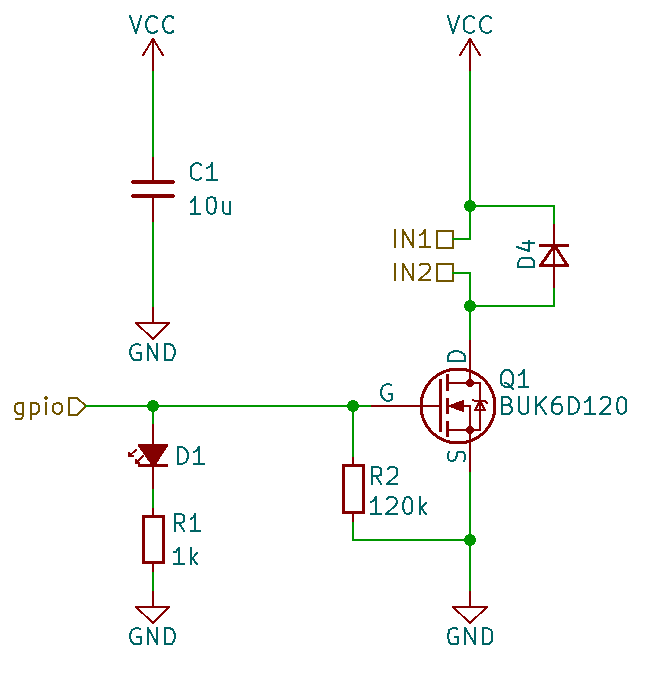
\includegraphics[width=0.5\linewidth]{transistor_circuit.png}
	\caption[Schematics for transistor part of the custom \gls{pcb}]{Schematics for transistor part of the custom \gls{pcb}}
	\label{fig:transistor_circuit}
\end{figure}

We took advantage of this custom \gls{pcb} to also test a specific transistor to see if it could handle the current in the coils. We used the BUK6D120 NMOS transistor.

It can handle a drain-source voltage of 40 V, and a temperature of 175°C.

We will power the coils with 5V and we can assume that they will be 1 ohm or more. This means that the absolute maximum current that can flow through the coils is 5A. But we will control it with a \gls{pwm} at 20\%, which means that the average current will be 1A.


We now know that we control the Gate of the NMOS with a 3V3 logic \gls{gpio} from the Raspberry Pi PICO. With a Gate Source Voltage of 3V3, we can expect a drain-source resistance of 0.28 ohm as seen in \ref{fig:transistor_rdson}.

\begin{figure}[H]
	\centering
	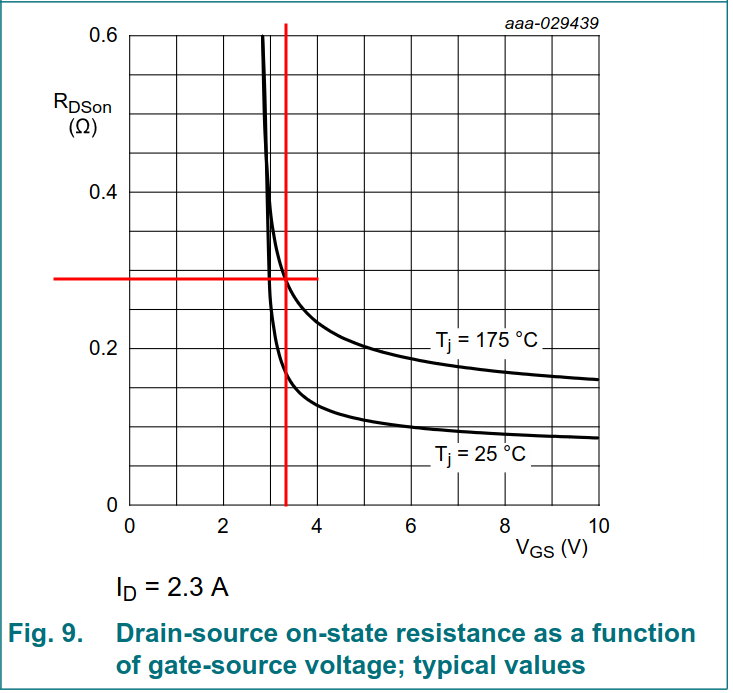
\includegraphics[width=0.7\linewidth]{transistor_rdson.png}
	\caption[BUK6D120 NMOS RDSon graph]{BUK6D120 NMOS RDSon graph}
	\label{fig:transistor_rdson}
\end{figure}

This means that the transistor will dissipate

$ P = I^2 * R => 1^2 * 0.28 = 0.28  Watts $

The thermal resistance from junction to ambient is maximum 76°C/W, which means that the temperature rise will be $ 0.28 * 76 = 21.28 $ °C of elevation for a constant current of 1A. This is easily manageable for the transistor.

\subsection{Coil designs}

The choice to have 4 coil designs was made not to have too big of a PCB while still testing different designs.

\subsubsection{Design 1 : Dual Linear coils}

The characteristics of the first design are:

\begin{itemize}
	\item 2 coils for each axis
	\item 10 mils (0.256mm) spacing between each traces
	\item 20 mils (0.508mm) width for the traces
\end{itemize}

\begin{figure}[H]
	\centering
	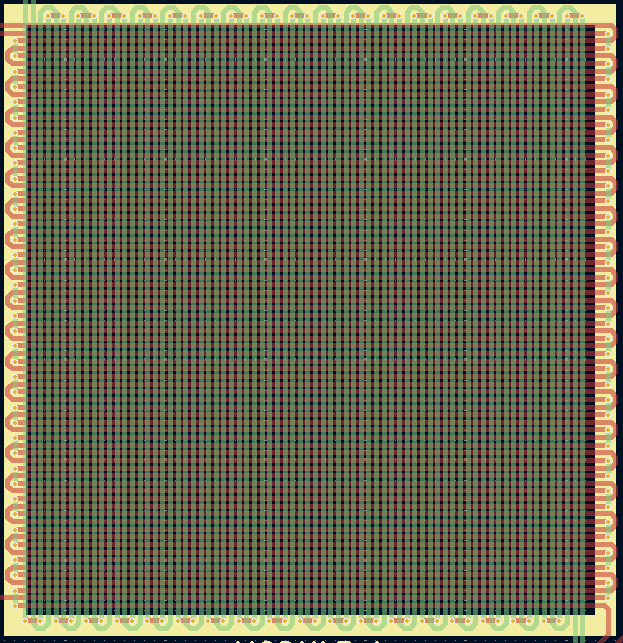
\includegraphics[width=0.6\linewidth]{design_1.png}
	\caption[Dual linear coils design]{Dual linear coils design}
	\label{fig:dual_linear}
\end{figure}

This design is not working as expected. The dual part of the design makes it impossible to have a magnet move in the same direction consitently because the order of the coils does not matter anymore since there is only 2 coils.

\subsubsection{Design 2 : Triple Linear coils}

The characteristics of the second design are:

\begin{itemize}
	\item 3 coils for each axis
	\item 10 mils (0.256mm) spacing between each traces
	\item 20 mils (0.508mm) width for the traces
\end{itemize}

\begin{figure}[H]
	\centering
	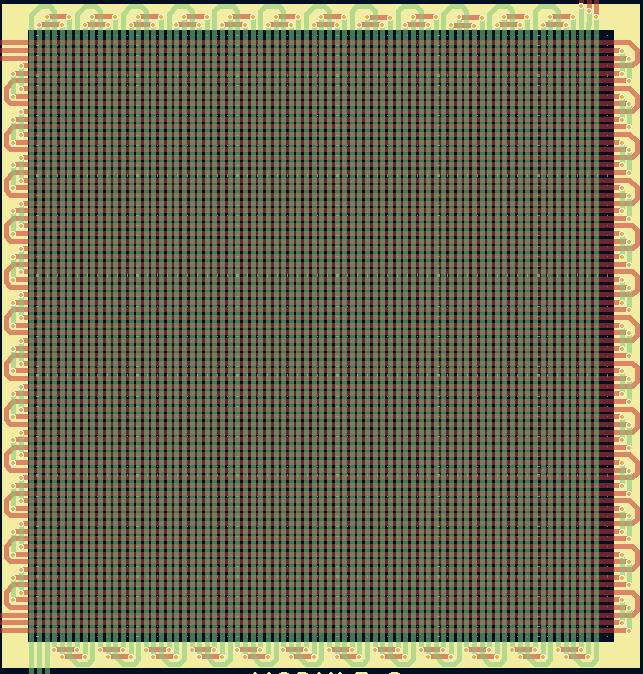
\includegraphics[width=0.6\linewidth]{design_2.png}
	\caption[Triple linear coils design]{Triple linear coils design}
	\label{fig:triple_linear}
\end{figure}

The design is pretty similar to the Pemi Technology design and is working relatively similar. The main changes have actually been the \gls{pcb} layers since we switched to 4 layers and have routed the traces on the first top ones. Switching to 4 layers changes the stackup so the first 2 layers are closer to the top, thus closer to the magnet. The magnet can move in both direction but is still stuck sometimes. The magnet is moving in the same axis as the top layer of the \gls{pcb}.

\newpage

\subsubsection{Design 3 : Circular coils}

This design is closer to the spiral coil design from Carl Bugeja. The characteristics of this third design are:

\begin{itemize}
	\item 2 layers
	\item 10 mils (0.256mm) trace width
	\item 5 mils (0.128mm) spacing traces
	\item 20mm diameter
	\item 25 turns
\end{itemize}

\begin{figure}[H]
	\centering
	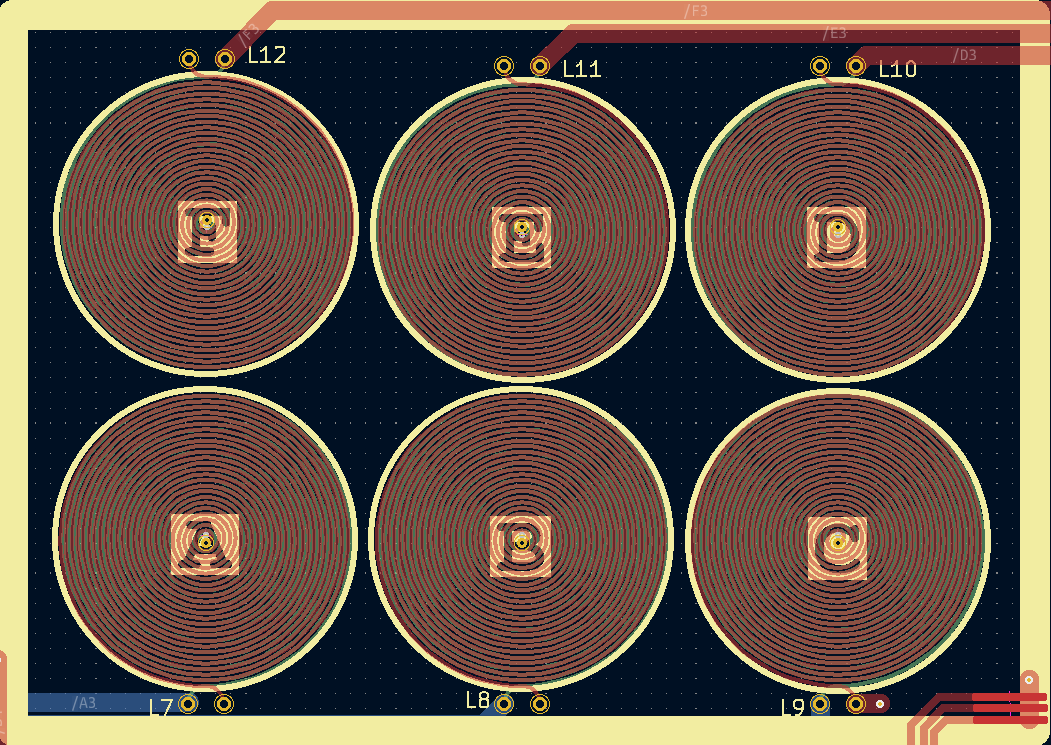
\includegraphics[width=0.6\linewidth]{design_3.png}
	\caption[Circular coils design]{Circular coils design}
	\label{fig:circular}
\end{figure}

This was the most promising design since the magnet was beig attracted to the center of the coil from the border of the spiral. But the magnetic field was not strong enough to move a magnet from a coil to the other.

\newpage


\subsubsection{Design 4 : Circular coils with more turns}

This design is quite similar to the third one but with thinner traces and thinner spacing thus making more turns. The characteristics of this fourth design are:

\begin{itemize}
	\item 2 layers
	\item 3.5 mils (0.089mm) trace width
	\item 3.5 mils (0.089mm) spacing traces
	\item 20mm diameter
	\item 50 turns
\end{itemize}

\begin{figure}[H]
	\centering
	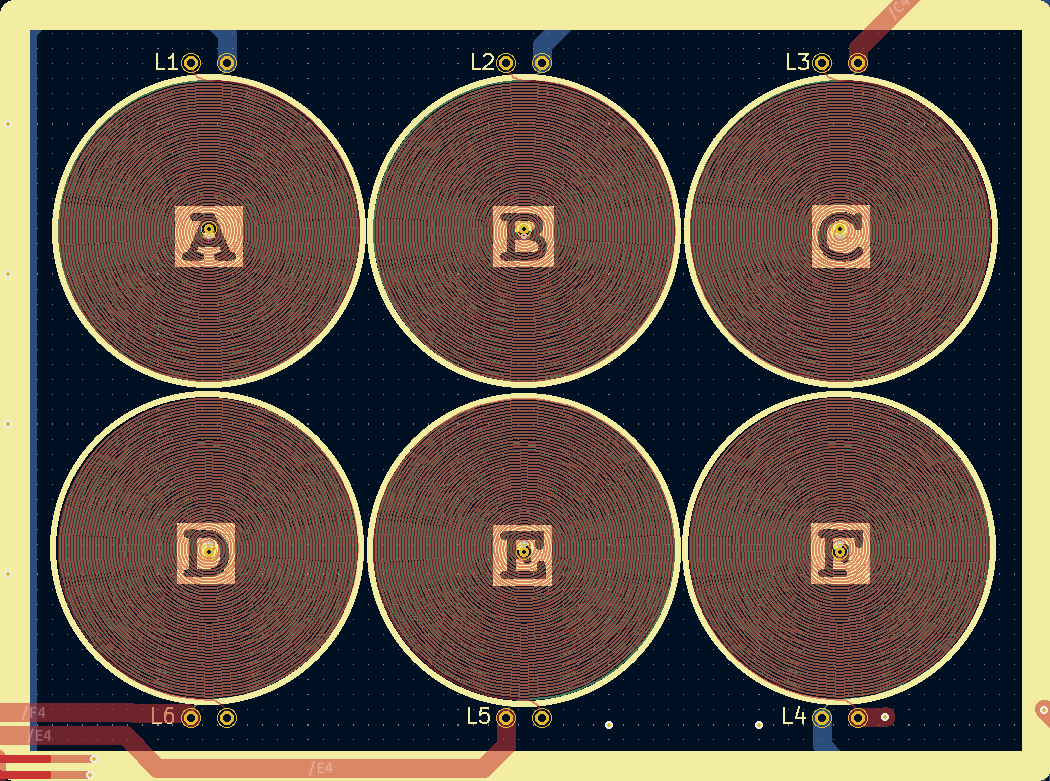
\includegraphics[width=0.6\linewidth]{design_4.png}
	\caption[Circular coils with more turns]{Circular coils with more turns}
	\label{fig:circular_more_turns}
\end{figure}

This final design should have given us a stronger magnetic for the same current, but with these small traces, the resistance was too high and the current was not enough to move a magnet.

\newpage


\section{Stand alone coil \gls{pcb}s}

These designs were not working perfectly so we went back to the drawing board and got some new designs on smaller \gls{pcb} controlled by the custom board drivers. We only needed to have the designs and some pins to connect to the driver board.
\\

We went for 3 different designs:
\begin{itemize}
	\item 4 layer circular coils to double de strength of the magnetic field of the third previous design
	\item 2x2 layer Circular interlaced coils to have a sub-coil closer between each main coil
	\item 2x2 layer rectangular interlaced coils to have a sub-coil closer between each main coil
\end{itemize}

\subsection{4 Layer circular coils}

This design has the same characteristics as the third previous design but with 4 layers of coil instead of 2. This should almost double the magnetic field strength.

\begin{figure}[H]
	\centering
	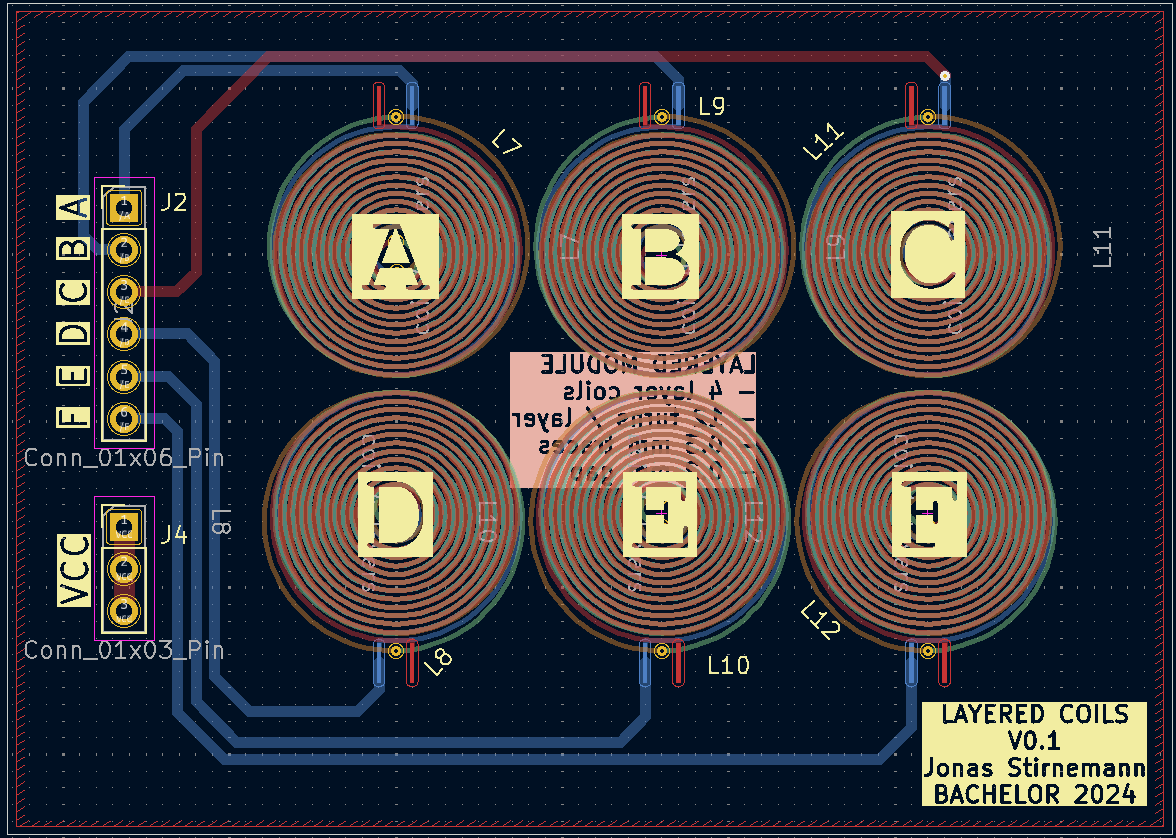
\includegraphics[width=0.6\linewidth]{4_layer_circular.png}
	\caption[4 layer circular coils design]{4 layer circular coils design}
	\label{fig:4_layer_circular}
\end{figure}

\begin{figure}[H]
	\centering
	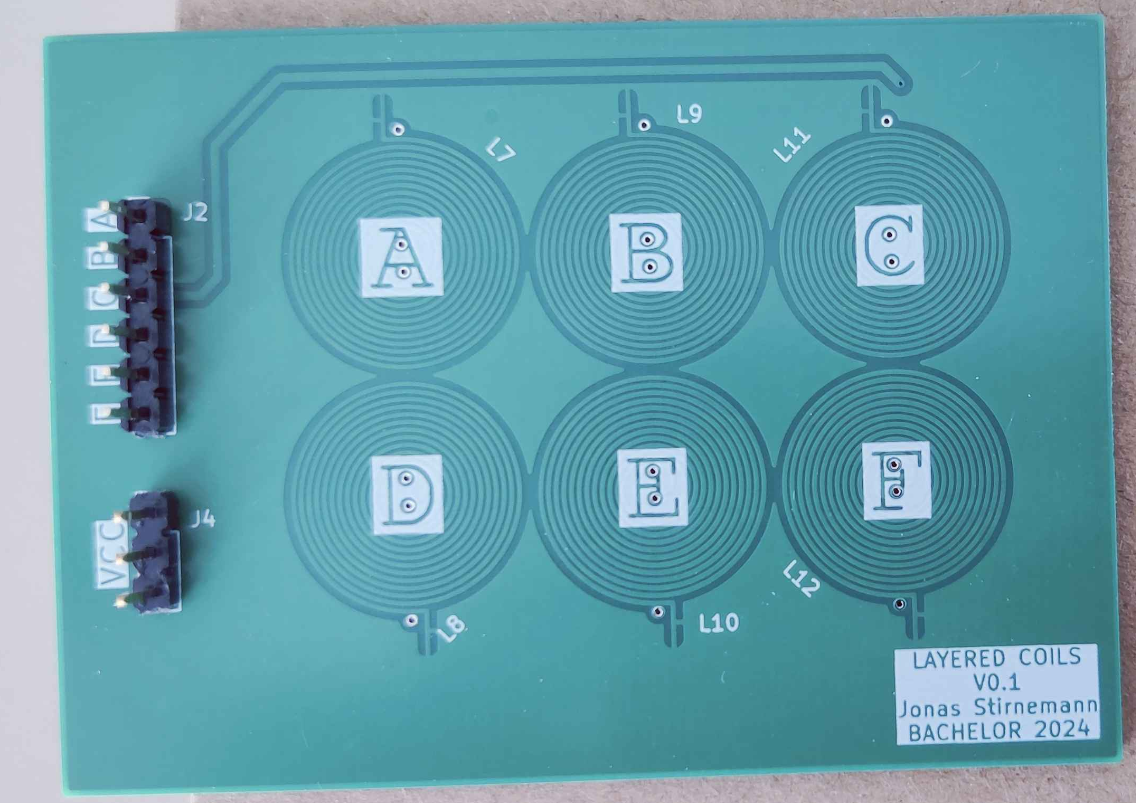
\includegraphics[width=0.6\linewidth]{4_layer_circular_pcb.png}
	\caption[4 layer circular \gls{pcb}]{4 layer circular \gls{pcb}}
	\label{fig:4_layer_circular_pcb}
\end{figure}



This was not working as expected, the magnet could still not jump from one coil to the other, the doubling of the magnetic field was not enough to move the magnet.

\newpage

\subsection{2x2 layers - Circular interlaced coils}

This design has a small trick to get multiple coils to overlap each other. On the 4 layer stackup we have a coil on the top layer and the inner second layer and the second coil on the first inner layer and the bottom layer. This way, we can have the coils overlapping and it's easier to move the magnet from one coil to the other.


\begin{figure}[H]
	\centering
	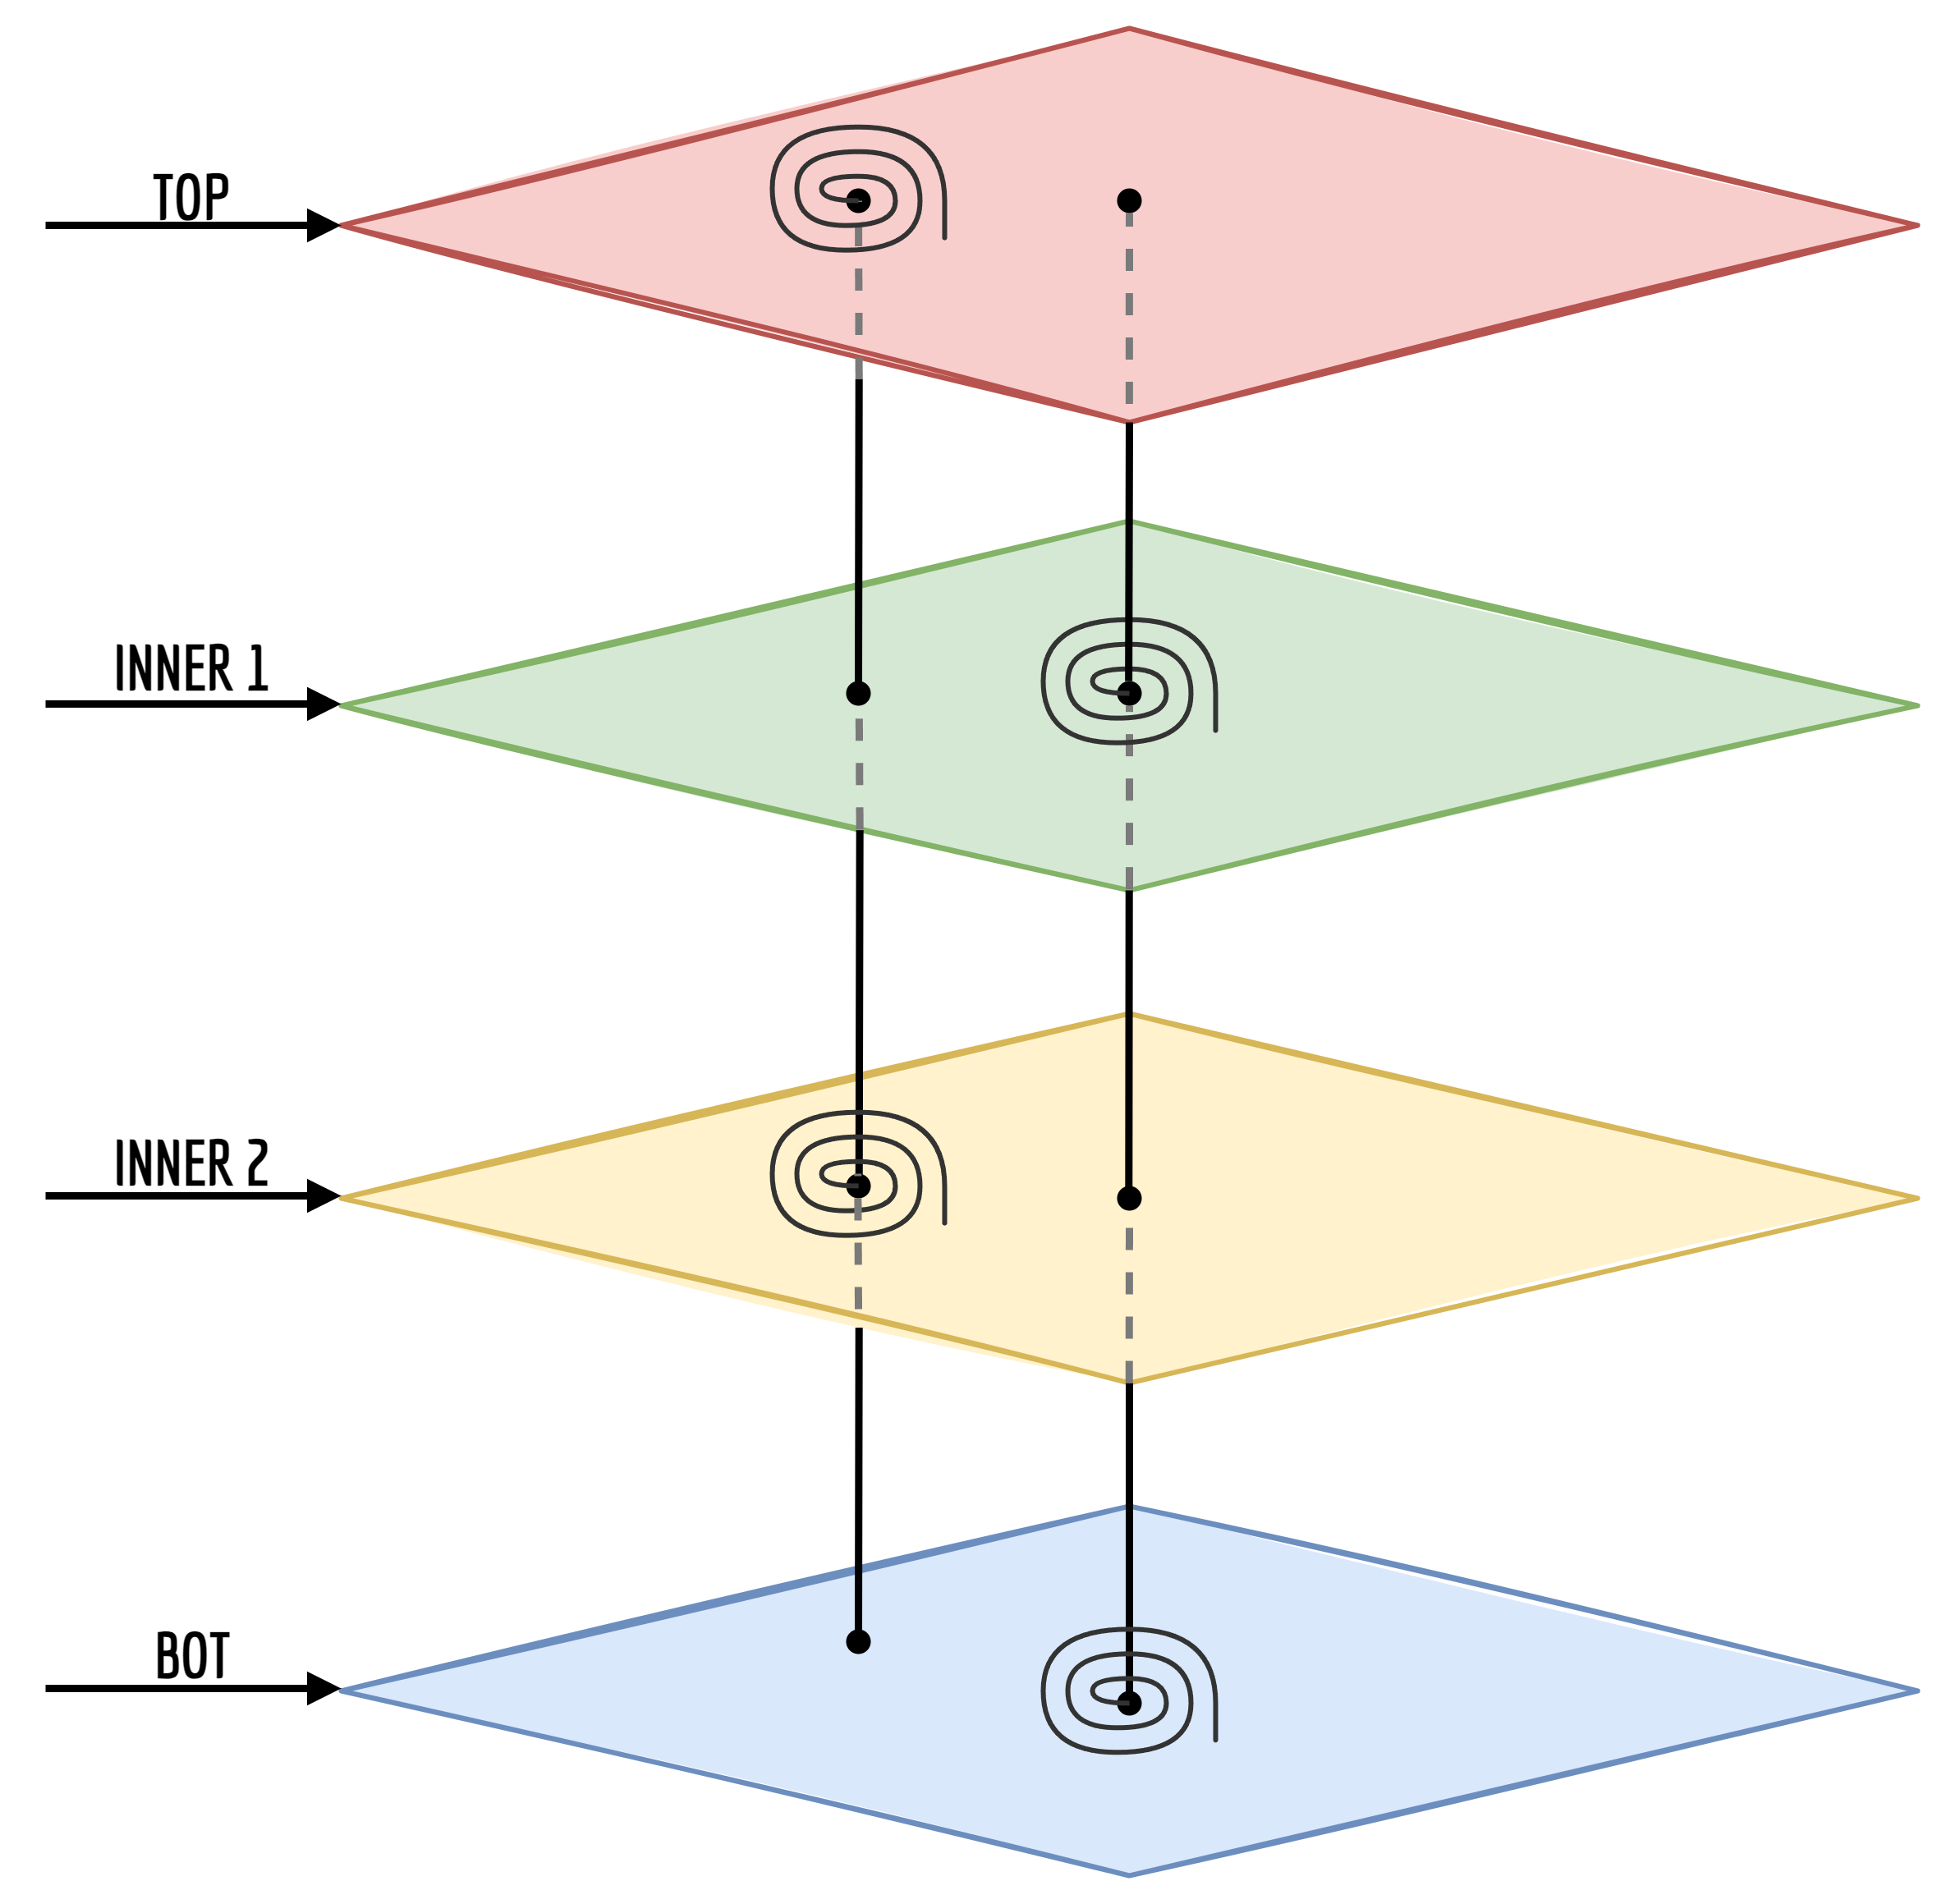
\includegraphics[width=0.6\linewidth]{stackup_circles.png}
	\caption[\gls{pcb} Stackup 4 layer overlap]{\gls{pcb} Stackup 4 layer overlap}
	\label{fig:stackup_circles}
\end{figure}

One issue with this shape is that it's hard to have them overlap on the 4 sides when being the same diameter, so we had to make smaller coils for the sub-coils. The center of the coils is where the force is the strongest, so we need the center of the coils to be as close as possible from each other.

\begin{figure}[H]
	\centering
	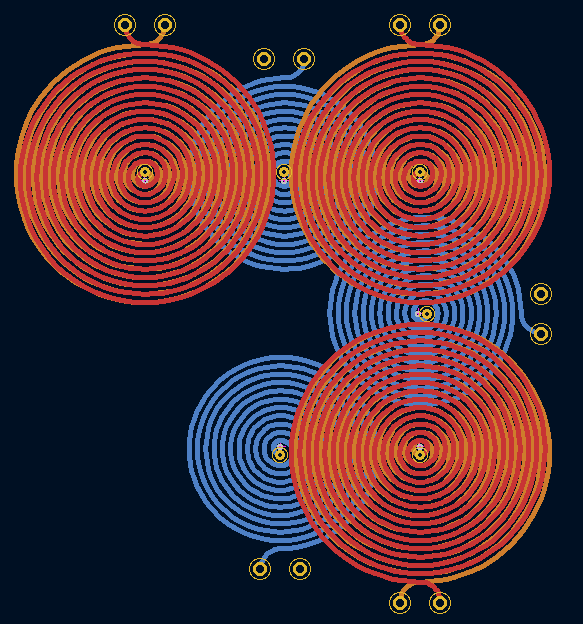
\includegraphics[width=0.6\linewidth]{smaller_coils.png}
	\caption[Circular sub coils are smaller]{Circular sub coils are smaller}
	\label{fig:smaller_coils}
\end{figure}

\begin{figure}[H]
	\centering
	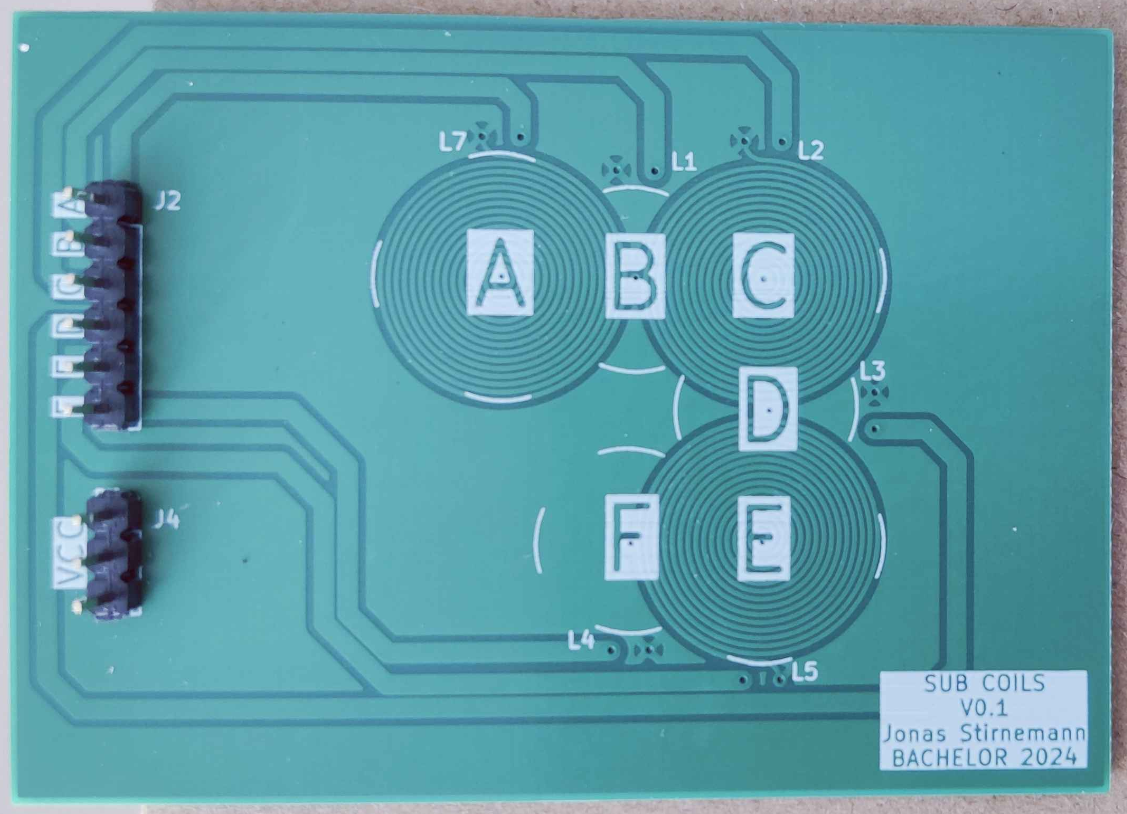
\includegraphics[width=0.6\linewidth]{sub_circular_pcb.png}
	\caption[Circular sub-coils \gls{pcb}]{Circular sub-coils \gls{pcb}}
	\label{fig:sub_circular_pcb}
\end{figure}

While promising, this design turned out to have it's sub coils too small to be powerfull enough to move a magnets between coils. The issue comes from the circular shapes that are difficult to have them overlap on the 4 sides of the main circle.

\newpage


\subsection{2x2 layers - Rectangular interlaced coils}

This design is similar to the previous one but with rectangular coils. This way we can have the coils overlap on the 4 sides of the main coil while still being the same size as the main.

The stackup is the same, the top layer and the inner second layer have the first coil and the first inner layer and the bottom layer have the second coil.

\begin{figure}[H]
	\centering
	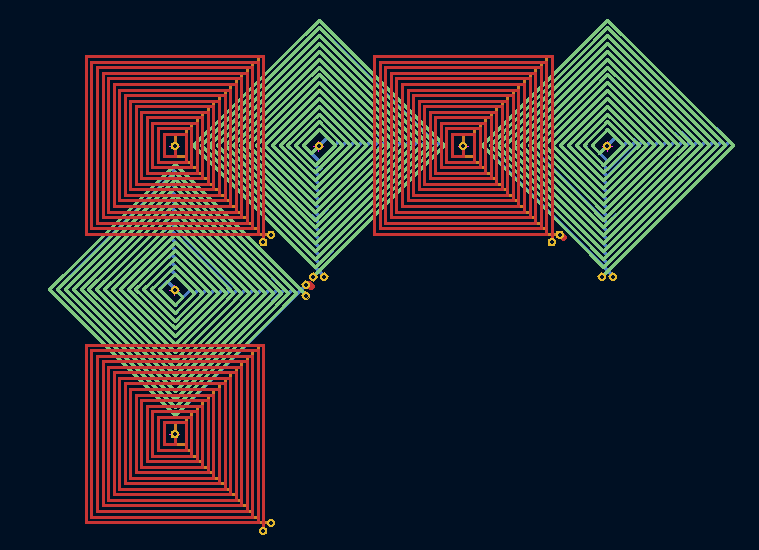
\includegraphics[width=0.7\linewidth]{square_design.png}
	\caption[Squares 4 layer overlap]{squares Stackup 4 layer overlap}
	\label{fig:square_design}
\end{figure}

\begin{figure}[H]
	\centering
	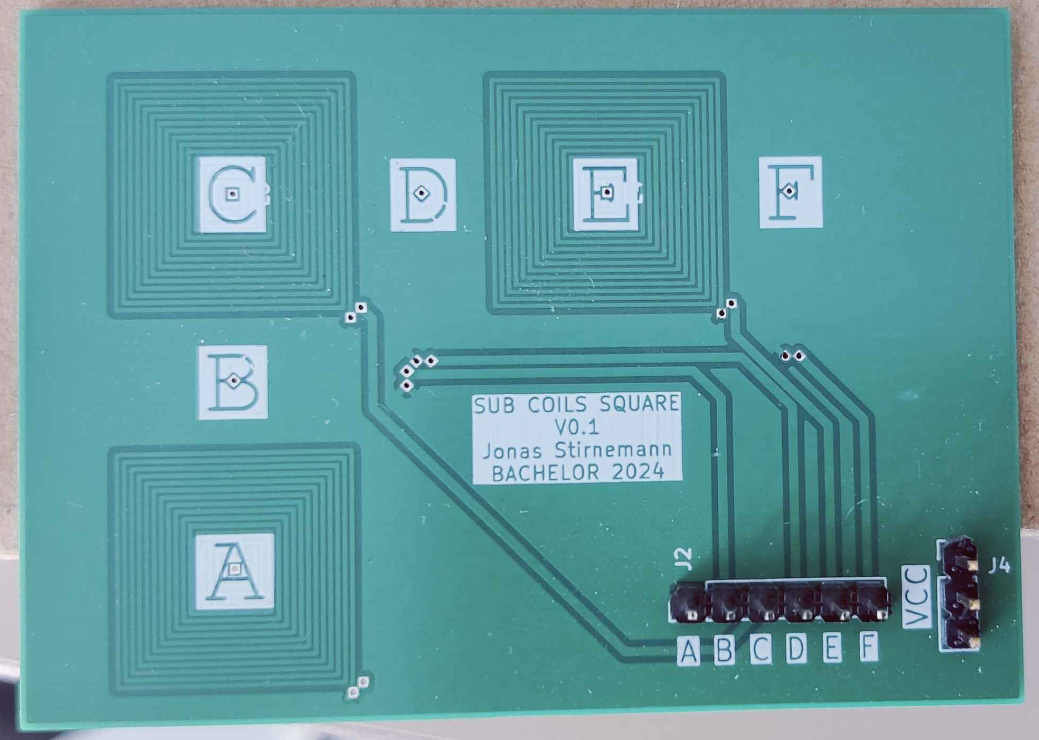
\includegraphics[width=0.7\linewidth]{square_pcb.png}
	\caption[Square sub-coils \gls{pcb}]{Square sub-coils \gls{pcb}}
	\label{fig:square_pcb}
\end{figure}

This design was the most promising, I made a 10mm magnet move back and fourth between the coils, it was heating up because the coils were being activated almost all the time, but from what i gathered with the thermal camera, the maximum heating we had was 70°C which is clearly still manageable for the \gls{pcb} and the magnet.